\newpage
\section[Фигура 2]{Фигура 2}

Строим эллипс. 
Дублируем эллипс, выделяем пару полученных фигур, также дублируем и осуществляем поворот.
Применяем инструмент \textit{\textbf{Interpolate}}.
Накладываем полученные фигуры друг на друга
\vspace{12pt}

Ниже приведены этапы применения изменений:
\begin{figure}[H]
    \begin{minipage}[h]{1\linewidth}
        \center{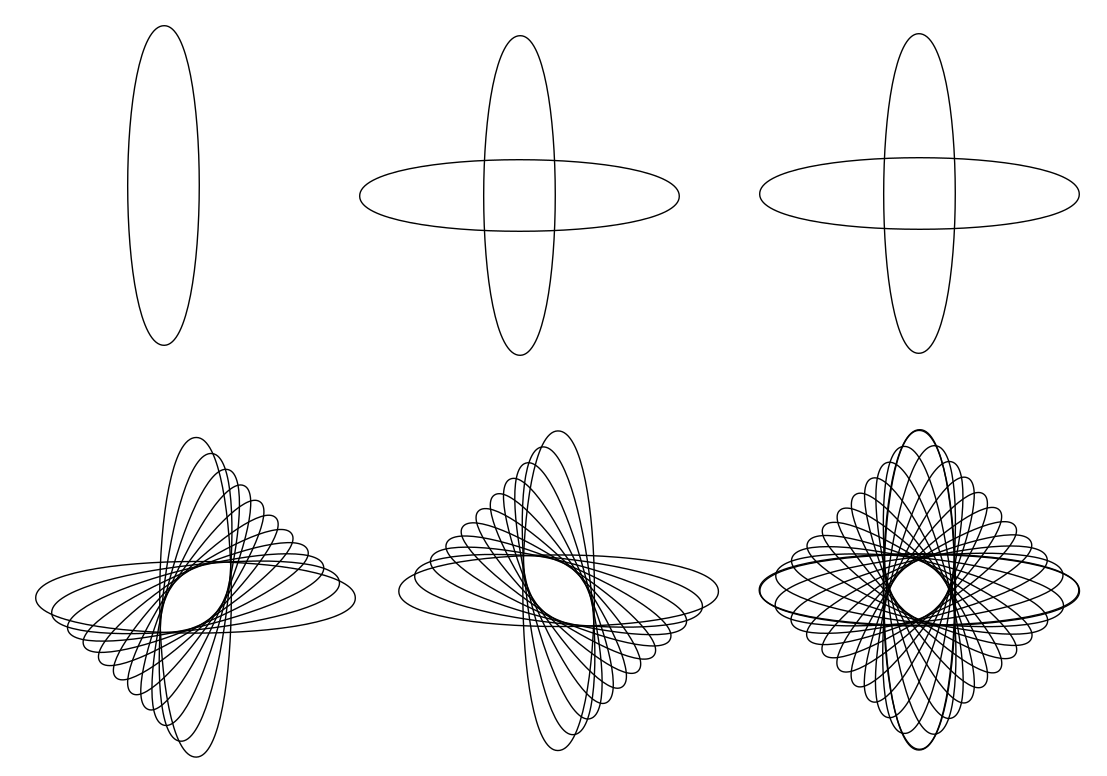
\includegraphics[width=1\linewidth]{2_pic.png}}
    \end{minipage}
\end{figure}
